\documentclass[11pt,a4paper,DIV12]{scrartcl}
\usepackage{amsmath}
\usepackage{amssymb}	
\usepackage{graphicx} 
\usepackage{multicol}
\usepackage[compat=1.1.0]{tikz-feynman}

\title{Diagrams}

\begin{document}
\maketitle
\centering

\begin{minipage}[]{0.32\textwidth}
\begin{minipage}[]{\textwidth}
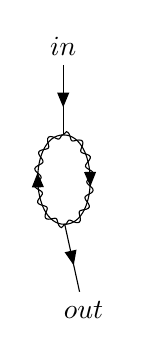
\begin{tikzpicture}
\begin{feynman}
\diagram[small]{
   i1 [particle=$in$] -- [fermion] v1,
   v1 -- [fermion, out=90, in=90, relative=true, looseness=1] v2,
   v1 -- [photon,  out=-90, in=-90, relative=true, looseness=1] v2,
   v2 -- [fermion, out=90, in=90, relative=true, looseness=1] v1,
   v2 -- [photon, out=-90, in=-90, relative=true, looseness=1] v1,
   v2 -- [fermion] o2 [particle=$out$], 
};
\end{feynman}
\end{tikzpicture}
\end{minipage}

\begin{minipage}[]{\textwidth}
\begin{center}
\# $1$\\ 
(symmetry: $-1$)
\end{center}
\end{minipage}

\vspace{1em}
\end{minipage}
%
\begin{minipage}[]{0.32\textwidth}
\begin{minipage}[]{\textwidth}
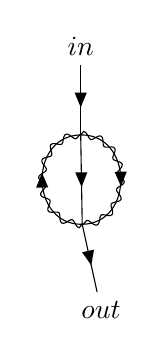
\begin{tikzpicture}
\begin{feynman}
\diagram[small]{
   i1 [particle=$in$] -- [fermion] v1,
   v1 -- [fermion, out=90, in=90, relative=true, looseness=1.5] v2,
   v1 -- [photon,  out=-90, in=-90, relative=true, looseness=1.5] v2,
   v1 -- [fermion,                relative=true] v2,
   v2 -- [fermion, out=90, in=90, relative=true, looseness=1.5] v1,
   v2 -- [photon, out=-90, in=-90, relative=true, looseness=1.5] v1,
   v2 -- [fermion] o2 [particle=$out$], 
};
\end{feynman}
\end{tikzpicture}
\end{minipage}

\begin{minipage}[]{\textwidth}
\begin{center}
\# $2$\\ 
(symmetry: $+1/2$)
\end{center}
\end{minipage}

\vspace{1em}
\end{minipage}
%
\begin{minipage}[]{0.32\textwidth}
\begin{minipage}[]{\textwidth}
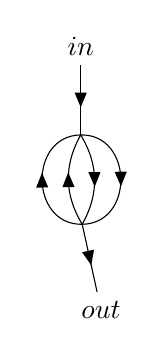
\begin{tikzpicture}
\begin{feynman} 
\diagram[small]{
   i1 [particle=$in$] -- [fermion] v1,
   v1 -- [fermion, out=90, in=90, relative=true, looseness=1.5] v2,
   %v1 -- [photon,  out=-90, in=-90, relative=true, looseness=1.5] v2,
   v1 -- [fermion, out=30, in=150, relative=true, looseness=1] v2,
   %v1 -- [photon,  out=-45, in=-45, relative=true, looseness=1.5] v2,
   v2 -- [fermion, out=90, in=90, relative=true, looseness=1.5] v1,
   v2 -- [fermion, out=30, in=150, relative=true, looseness=1] v1,
   %v2 -- [photon, out=-90, in=-90, relative=true, looseness=1.5] v1,
   %v2 -- [fermion, out=45, in=45, relative=true, looseness=1.5] v1,
   %v2 -- [photon, out=-45, in=-45, relative=true, looseness=1.5] v1,
   v2 -- [fermion] o2 [particle=$out$], 
};
\end{feynman}
\end{tikzpicture}
\end{minipage}

\begin{minipage}[]{\textwidth}
\begin{center}
\# $3$\\ 
(symmetry: $+1$)
\end{center}
\end{minipage}

\vspace{1em}
\end{minipage}
%
%
\begin{minipage}[]{0.32\textwidth}
\begin{minipage}[]{\textwidth}
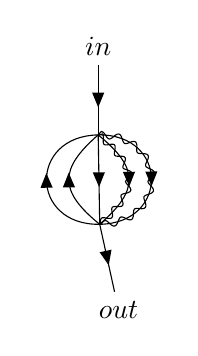
\begin{tikzpicture}
\begin{feynman} 
\diagram[small]{
   i1 [particle=$in$] -- [fermion] v1,
   v1 -- [fermion, out=90,  in=90,   relative=true, looseness=2] v2,
   v1 -- [fermion, out=50,  in=130,  relative=true, looseness=1.5] v2,
   v2 -- [boson,   out=-90, in=-90,  relative=true, looseness=2] v1,
   v2 -- [boson,   out=-50, in=-130, relative=true, looseness=1.5] v1,
   v1 -- [fermion] v2,
   v2 -- [fermion, out=50, in=130, relative=true, looseness=1.5] v1,
   v2 -- [fermion, out=90, in=90, relative=true, looseness=2] v1,
   v2 -- [fermion] o2 [particle=$out$], 
};
\end{feynman}
\end{tikzpicture}
\end{minipage}

\begin{minipage}[]{\textwidth}
\begin{center}
\# $4$\\ 
(symmetry: $+1$)
\end{center}
\end{minipage}

\vspace{1em}
\end{minipage}
%
\begin{minipage}[]{0.32\textwidth}
\begin{minipage}[]{\textwidth}
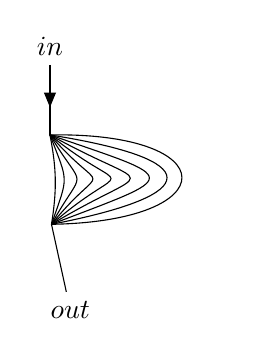
\begin{tikzpicture}
\begin{feynman} 
\diagram[small]{
   i1 [particle=$in$] -- [fermion] v1,
   v1 -- [plain, out=90, in=90,  relative=true, looseness=5.0] v2,
   v1 -- [plain, out=80, in=100, relative=true, looseness=4.5] v2,
   v1 -- [plain, out=70, in=110, relative=true, looseness=4.0] v2,
   v1 -- [plain, out=60, in=120, relative=true, looseness=3.5] v2,
   v1 -- [plain, out=50, in=130, relative=true, looseness=3.0] v2,
   v1 -- [plain, out=40, in=140, relative=true, looseness=2.5] v2,
   v1 -- [plain, out=30, in=150, relative=true, looseness=2.0] v2,
   v1 -- [plain, out=20, in=160, relative=true, looseness=1.5] v2,
   v1 -- [plain, out=10, in=170, relative=true, looseness=1.0] v2,
   v2 -- [plain] o2 [particle=$out$], 
};
\end{feynman}
\end{tikzpicture}
\end{minipage}

\begin{minipage}[]{\textwidth}
\begin{center}
\# $5$\\ 
(symmetry: $+1$)
\end{center}
\end{minipage}

\vspace{1em}
\end{minipage}
%
\begin{minipage}[]{0.32\textwidth}
\begin{minipage}[]{\textwidth}
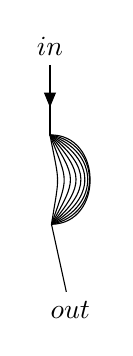
\begin{tikzpicture}
\begin{feynman} 
\diagram[small]{
   i1 [particle=$in$] -- [fermion] v1,
   v1 -- [plain, out=90, in=90,  relative=true, looseness=1.5] v2,
   v1 -- [plain, out=80, in=100, relative=true, looseness=1.5] v2,
   v1 -- [plain, out=70, in=110, relative=true, looseness=1.5] v2,
   v1 -- [plain, out=60, in=120, relative=true, looseness=1.5] v2,
   v1 -- [plain, out=50, in=130, relative=true, looseness=1.5] v2,
   v1 -- [plain, out=40, in=140, relative=true, looseness=1.5] v2,
   v1 -- [plain, out=30, in=150, relative=true, looseness=1.5] v2,
   v1 -- [plain, out=20, in=160, relative=true, looseness=1.5] v2,
   v1 -- [plain, out=10, in=170, relative=true, looseness=1.5] v2,
   v2 -- [plain] o2 [particle=$out$], 
};
\end{feynman}
\end{tikzpicture}
\end{minipage}

\begin{minipage}[]{\textwidth}
\begin{center}
\# $5$\\ 
(symmetry: $+1$)
\end{center}
\end{minipage}

\vspace{1em}
\end{minipage}
%
\end{document}
